\documentclass[11pt,largemargins]{homework}
\usepackage{xeCJK}
\usepackage{amsthm}
\usepackage{amsmath}

\usepackage{tikz}
\usetikzlibrary{calc}
\usepackage{amsmath,amssymb}
\usepackage{tikz-cd}
\usetikzlibrary{fit}
\usetikzlibrary{arrows.meta}
\usepackage{enumitem}


\newcommand{\hwname}{蘇則宇}
\newcommand{\hwemail}{B11201005}
\newcommand{\hwtype}{Homework}
\newcommand{\hwnum}{10}
\newcommand{\hwclass}{Modern Algebra I}
\newcommand{\hwlecture}{}
\newcommand{\hwsection}{}

% This is just used to generate filler content. You don't need it in an actual
% homework!
\usepackage{lipsum}
\begin{document}
	\maketitle
	\question
	Consider 
	\begin{center}
		\begin{tikzpicture}
			\node (A1) at (0,0){$A^i$};
			\node (B1) at (2,0){$B^i$};
			\node (C1) at (4,0){$C^i$};
			\node (A2) at (0,-1.5){$A^{i+1}$};
			\node (B2) at (2,-1.5){$B^{i+1}$};
			\node (C2) at (4,-1.5){$C^{i+1}$};
			
			\draw[->] (A1)--(A2) node[midway,left]{$a_i$};
			\draw[->] (B1)--(B2) node[midway,left]{$b_i$};
			\draw[->] (C1)--(C2) node[midway,left]{$c_i$};
			
			\coordinate (O1) at (0,1.5);
			\draw[->] (O1)--(A1);
			\coordinate (O2) at (2,1.5);
			\draw[->] (O2)--(B1);
			\coordinate (O3) at (4,1.5);
			\draw[->] (O3)--(C1);
			
			\node (LU) at (-2,0){0};
			\draw[->] (LU)--(A1);
			\node (LD) at (-2,-1.5){0};
			\draw[->] (LD)--(A2);
			\node (RU) at (6,0){0};
			\draw[->] (C1)--(RU);
			\node (RD) at (6,-1.5){0};
			\draw[->] (C2)--(RD);
			
			\draw[->] (A1)--(B1) node[midway,above]{$f^i$};
			\draw[->] (B1)--(C1)
			node[midway,above]{$g^i$};
			\draw[->] (A2)--(B2)
			node[midway,above]{$f^{i+1}$};
			\draw[->] (B2)--(C2)
			node[midway,above]{$g^{i+1}$};
			
			\coordinate (o1) at (0,-3);
			\draw[->] (A2)--(o1);
			\coordinate (o2) at (2,-3);
			\draw[->] (B2)--(o2);
			\coordinate (o3) at (4,-3);
			\draw[->] (C2)--(o3);
		\end{tikzpicture}
	\end{center}
	Then we have:
	\begin{center}
		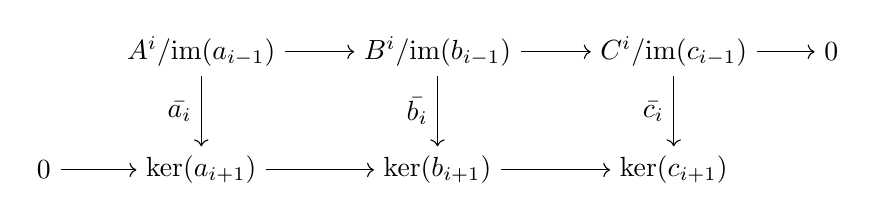
\begin{tikzpicture}
			\node (A) at (0,0) {$A^i/\text{im}(a_{i-1})$};
			\node (B) at (3,0) {$B^i/\text{im}(b_{i-1})$};
			\node (C) at (6,0) {$C^i/\text{im}(c_{i-1})$};
			\node (Z1) at (0,-1.5) {$\text{ker}(a_{i+1})$};
			\node (Z2) at (3,-1.5) {$\text{ker}(b_{i+1})$};
			\node (Z3) at (6,-1.5) {$\text{ker}(c_{i+1})$};
			\node (R) at (8,0){$0$};
			\node (L) at (-2,-1.5){$0$};
			
			\draw[->] (A)--(B);
			\draw[->] (B)--(C);
			\draw[->] (C)--(R);
			\draw[->] (L)--(Z1);
			\draw[->] (Z1)--(Z2);
			\draw[->] (Z2)--(Z3);
			\draw[->] (A)--(Z1) node[midway,left]{$\bar{a_i}$};
			\draw[->] (B)--(Z2) node[midway,left]{$\bar{b_i}$};
			\draw[->] (C)--(Z3) node[midway,left]{$\bar{c_i}$};
		\end{tikzpicture}
	\end{center}
	Observe that $\text{ker}(\bar{a_i})=\text{ker}(a_i)/\text{im}(a_{i-1})=H^i(A)$, and coker$(\bar{a_i})=\text{im}(a_i)/\text{ker}(a_{i+1})=H^{i+1}(A)$. Apply Snake Lemma, done.
\question

$(a)\Rightarrow(b)$ has been proved in class.\\
$(b)\Rightarrow(a):$ Let $M$ be projective, then it is a direct summand of some free $A-$module $F$, hence a submodule of $F$. But submodules of a free module over PID is also free, hence $M$ is free.\\
$(a)\Rightarrow (c):$ It suffices to show $A$ as a $A-$mod is trosion-free. Since $A$ is a domain, done.\\
$(c)\Rightarrow (a):$ Need an additional assumption: $M$ is finitely generated. ($\mathbb{Q}$ is torsion-free but not free)\\
Assume $M$ is f.g., then by Fundamental Theorem of Finitely Generated Module over PID, $M\cong A^n\oplus A/(a_1)\oplus A/(d_2)\oplus ... \oplus A/(d_t)$. Since $M$ is torsion-free, the torsion part $A/(a_1)\oplus A/(d_2)\oplus ... \oplus A/(d_t)$ is zero hence $M\cong A^n$ is free.\\
\question
\begin{enumerate}[label=(\alph*)]
	\item
Let 
\begin{equation*}
	0\rightarrow I^0\rightarrow I^1\rightarrow ...
\end{equation*}
be an injective resolution of $N$, then there's an exact sequence:
\begin{equation*}
	0\rightarrow N\xrightarrow{\iota} I^0\xrightarrow{d^0} I^1\xrightarrow{d^1} ...
\end{equation*}
Apply Hom functor $\text{Hom}_A(M,-)$ to the above chains:
\begin{equation*}
	0\rightarrow
	 \text{Hom}(M,I^0)\xrightarrow{\text{Hom}(M,d^0)} \text{Hom}(M,I^1)\xrightarrow{\text{Hom}(M,d^1)} ...
\end{equation*}
\begin{equation*}
	0\rightarrow
	\text{Hom}(M,N)\xrightarrow{\text{Hom}(M,\iota)} \text{Hom}(M,I^0)\xrightarrow{\text{Hom}(M,d^0)} \text{Hom}(M,I^1)\xrightarrow{\text{Hom}(M,d^1)} ...
\end{equation*}
The second chain is exact. To find $\text{Ext}_{A}^{i}(M,N)$, need to find the i-th cohomology of the first chain.


$\text{Ext}_{A}^{0}(M,N)=\text{ker(} \text{Hom}(M,d^0))$.
Since hom functor $\text{Hom}(M,-)$ preserve injection, $\text{ker(} \text{Hom}(M,d^0))=\text{im}(\text{Hom}(M,\iota))\cong \text{Hom}(M,N)$.
\item
Consider two injective resolutions $I^\bullet, J^\bullet$ of $N$, and identity map $id_N$. There is a chain map $f^\bullet$ from $I^\bullet$ to $J^\bullet$, and similarly, a chain map $g^\bullet$ from $J\bullet$ to $I^\bullet$.\\
Apply hom functor to both chain, then $f^\bullet,g^\bullet$ maps the n-th cohomology into n-th cohomology and $fg^\bullet=id^\bullet$, the identity in cohomology, hence a quasi-isomorphism. So the $\text{Ext}_{A}^{i}$ derivied in both injective resolution is isomorphic. 
\end{enumerate}
\end{document}